\documentclass[a4papaer]{article}
 
\usepackage{hyperref}
\usepackage[left=1.0cm,top=0.5cm,right=1.0cm,bottom=1.0cm]{geometry}
\usepackage[spanish, english]{babel}
\usepackage[utf8]{inputenc}
\usepackage{amsmath}
\usepackage{nccmath}
\usepackage{graphicx}
\usepackage[colorinlistoftodos]{todonotes}
\usepackage{amssymb}
\usepackage{listings}
\providecommand{\abs}[1]{\lvert#1\rvert}
 
 
\begin{document}
 
\title{Laboratorio 3 Redes de Computadores}
\author{Diego Muñoz - 201073572-9 - diego.munozd@alumnos.usm.cl}
\date{20 de Junio de 2014}
\maketitle
 
\section{Introducción}
 
La resolución de este trabajo se hizo completamente en Latex, desarrollando manualmente los ejercicioes, asi, evitando codigo en python.
 
\section{Usando OVT}
 
Para el desarrollo de esta sección, se utilizó un simil a la aplicacion Open Visual Traceroute, debido a que no se encontraba disponible para MacOSX, esta aplicación se llama Visualroute y se puede encontrar en $http://www.visualware.com/$.

Es sabido que las conexiones intercontinentales son mediante cables submarinos ($http://www.submarinecablemap.com/$), por lo que notaremos que todas las direcciones que probamos en esta tarea primero salen de Chile a Estados Unidos independiente del destino final que estos tengan, esto es debido a que no existe conexion directa con Australia por ejemplo. \\

Esto lo podemos ver en el capítulo 1 del ramo, en donde nos hablan de niveles de redes de internet, donde aparecen ISP1 e ISP2 para conexiones nacionales e internacionales.

Ademas de la de Valparaiso, existe otra salida submarina en Arica, pero no se utilizará en esta tarea.

\subsection{http://moodle.inf.utfsm.cl/}

\begin{figure}[h]
  \centering
    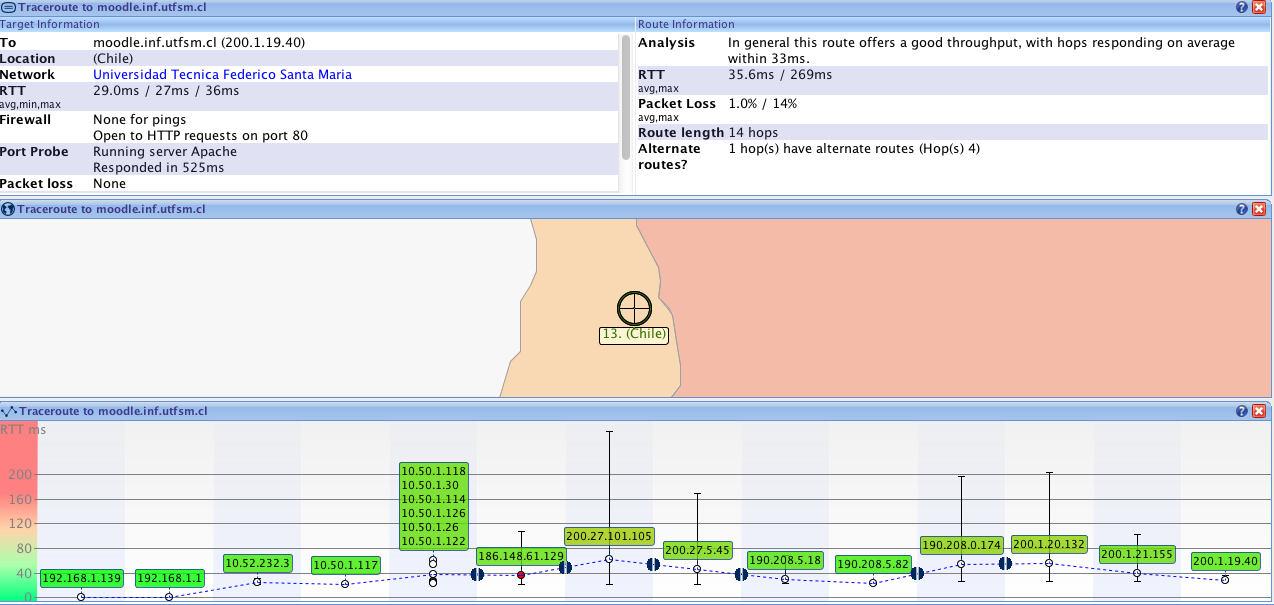
\includegraphics[width=1\textwidth]{ss1}
  \caption{Moodle}
  \label{fig:Trace Route de http://moodle.inf.utfsm.cl/}
\end{figure}


Es el caso ejemplificador de conexiones locales, notamos en la screen que ninguno de los hops por los que pasan los paquetes salen de Chile, esto es debido a que el servidor donde esta alojado Moodle se encuentra en Valparaiso, por lo que, los paquetes eligen la ruta mas óptima, que es manteniendos dentro del territorio nacional. Además podemos observar todos los tiempos de respuestas estan en color verde, lo que para la aplicación significa que son optimos, salvo los ultimos 2, que es cuando llegan a los routers en Valpariso que aumentan sus tiempos de respuesta un poco. En resumen, al encontrarse los servidores de destino en la misma red nacional, no requiere una conexión internacional.

\pagebreak

\subsection{http://cime.cl/}


\begin{figure}[h]
  \centering
    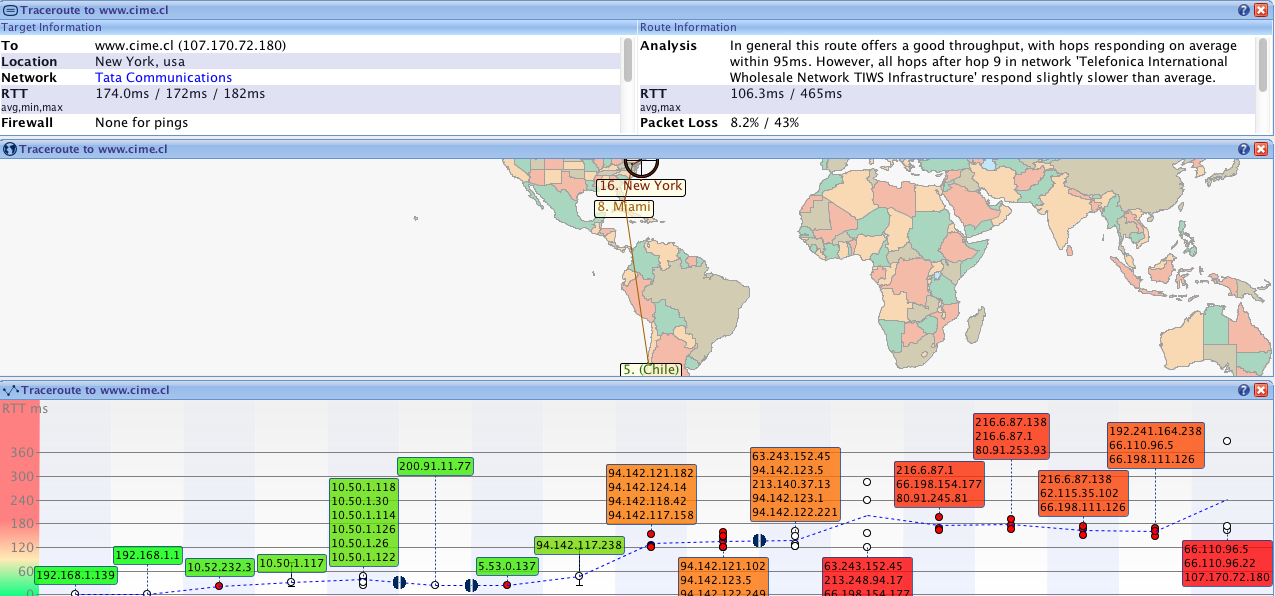
\includegraphics[width=1\textwidth]{ss2}
  \caption{Cime}
  \label{fig:Trace Route de http://cime.cl/}
\end{figure}



Para el caso de cime, notamos que los servidores se encuentran en Nueva York, USA. A diferencia de Moodle, la conexión debe salir de la red chilena y dirigirse a USA, para esto los paquetes llegan a Valparaiso, donde se encuentra la salida al cable submarino, y a travez del enlace internacional  \textbf{Telefónica International Wholesale Network Infrastructure} sale hacia Estados Unidos donde se reciben en Miami. Luego de llegado a USA es donde se complica un poco, porque dentro de este país existen muchas redes locales (ISP2), en la cuales los paquetes deben acceder dependiendo el servidor donde esten alojados. En este caso, $cime$ toma la rede \textbf{TATA Communications} hasta su llegada a Nueva York.
 
\begin{figure}[h]
  \centering
    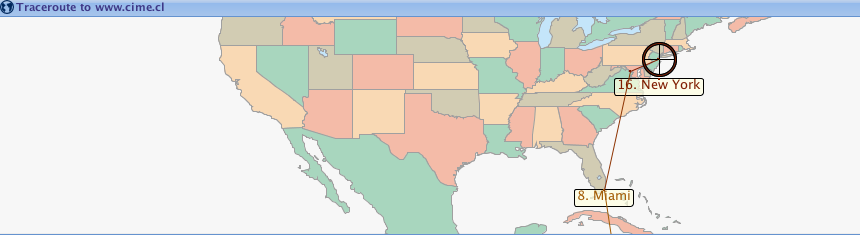
\includegraphics[width=1\textwidth]{ss3}
  \caption{Cime}
  \label{fig:Trace Route de http://cime.cl/}
\end{figure}


\pagebreak

\subsection{http://wikipedia.com/}

\begin{figure}[h]
  \centering
    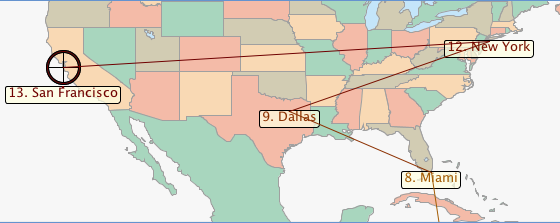
\includegraphics[width=1\textwidth]{ss5}
  \caption{Wikipedia}
  \label{fig:Trace Route de http://wikipedia.org/}
\end{figure}

Notamos que los servidores de Wikipedia estan alojados en la red Wikimedia en San Francisco, USA. Para llegar alla, al igual que en el caso de Cime que esta alojado en Nueva York, los paquetes viajan a travez de la red nacional hasta llegar al punto de salida en Valparaiso de \textbf{Telefónica International Wholesale Network Infrastructure}, llegando a la misma en Miami. Luego viajan hacia Dallas por la misma red, finalmente para llegar a una de las redes nacionales de USA \textbf{Tinet International Network}. 

\begin{figure}[h]
  \centering
    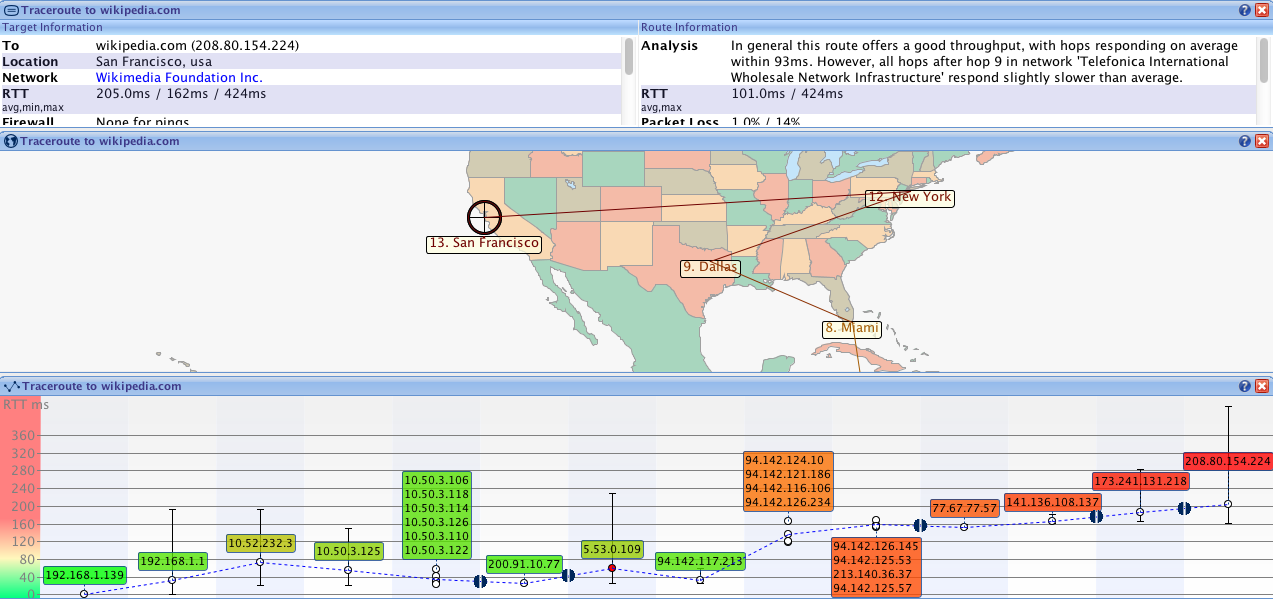
\includegraphics[width=1\textwidth]{ss4}
  \caption{Wikipedia}
  \label{fig:Trace Route de http://wikipedia.org/}
\end{figure}

Una vez mas, notar que los paquetes al salir de territorio nacional (hop 94.142.117.213), aumentan sus latencias en los tiempos de respuesta, mostrandose de color naranjo o rojo, aún después de escoger las mejores rutas.

\pagebreak

\subsection{http://www.chile.embassy.gov.au/}

\begin{figure}[h]
  \centering
    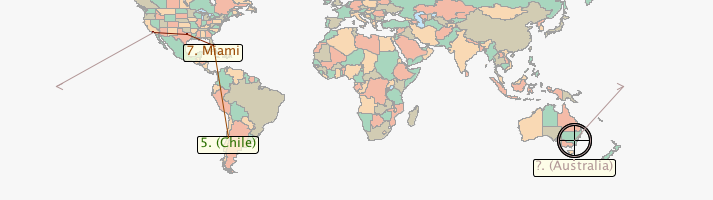
\includegraphics[width=1\textwidth]{au1}
  \caption{Embajada Australia en Chile}
  \label{fig:Trace Route de http://www.chile.embassy.gov.au/}
\end{figure}

A diferencia de los casos anteriores, los servidores de la embajada de Australia en Chile se encuentrán en Australia, por lo tanto, se observan algunos cambios en el camino por el cual los paquetes realizan su camino. Para llegar a Australia, no existe un enlace directo desde Chile, por lo que los paquetes generan su camino hacia Estados Unidos por la ruta de salida de Chile ya mencionada (Telefónica), luego pasa por la rede local de Estados Unidos, \textbf{Level 3 Communications, Inc} hasta la salida a un nuevo cable submarino que atravieza todo el Oceano Pácifico regido por la empresa \textbf{Pacnet Service (Japan)} hasta su llegada a Australia.

\begin{figure}[h]
  \centering
    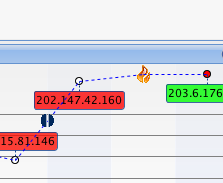
\includegraphics[width=0.5\textwidth]{au4}
  \caption{Embajada Australia en Chile}
  \label{fig:Trace Route de http://www.chile.embassy.gov.au/}
\end{figure}

En este punto notamos algo extraño, el programa no nos entrega información específica sobre donde llega, y esto es debido que al ser una página gubernamental y privada, utiliza firewalls que impiden el acceso completo a esta (notar imagen de una llamita). Es por esto que solo podemos saber que los paquetes llegan a este punto en Australia y después no sabemos que sucede con ellos.

\pagebreak

\begin{figure}[h]
  \centering
    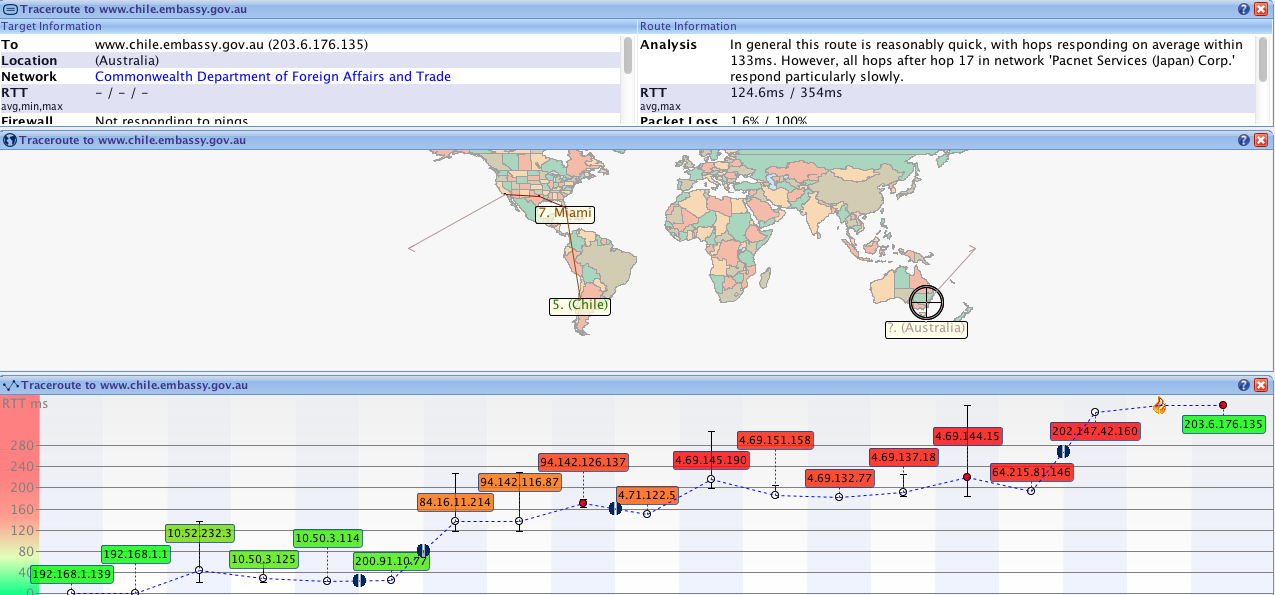
\includegraphics[width=1\textwidth]{au2}
  \caption{Embajada Australia en Chile}
  \label{fig:Trace Route de http://www.chile.embassy.gov.au/}
\end{figure}

Con respecto al camino que toman los paquetes, nuevamente, se observa que una vez fuera de territorio nacional, las latencias en los tiempos de respuesta aumenta (color naranja o rojo), a pesar de que se escoge la ruta menos congestionada.

\pagebreak

\subsection{http://google.cl/}

\begin{figure}[h]
  \centering
    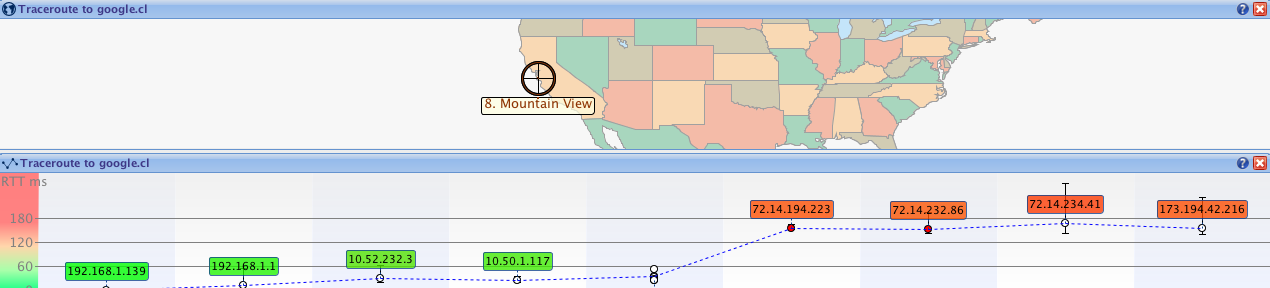
\includegraphics[width=1\textwidth]{g1}
  \caption{Google Chile}
  \label{fig:Trace Route de http://www.google.cl/}
\end{figure}

El enlace que se genera es directo hasta mountain view en Estados Unidos donde se alojan los servidores de Google, no pasa por intemermediarios, lo que hace presumir, que la conexion es inalambrica, y no pasa por cables submarinos.

\section{Algoritmo Vector-Distancia s/Cortes}
 
Para la realización de este ejercicio, se utilizó el agoritmo de $Bellman Ford$ y se modificó para que recorriera los diccionarios que genera e imprima en pantalla las tablas de cada router con sus costos. Notar que este algoritmo usa convergencia para finalizar cada iteracion de routers, por lo que se pueden apreciar tablas repetidas. Si se hiciese a mano, serian menos tablas, ya que se puede disernir facilmente cuando las tablas comienzan a repetirse.

De todas formas el código esta comentado.

La matriz final obtenida es:

\begin{table}[h]
\centering
\begin{tabular}{lclclclclclclclclclclc}

& PC & A & B & C & D & E & F & G & H & I & Server \\\hline\\
A&3&0&1&10&12&9&11&4&11&10&11 \\
B&4&1&0&9&11&8&10&5&12&9&10 \\
C&13&10&9&0&2&5&6&14&7&4&5 \\
D&15&12&11&2&0&3&4&12&5&2&3 \\
E&12&9&8&5&3&0&2&11&4&1&2 \\
F&14&11&10&6&4&2&0&13&6&3&4 \\
G&7&4&5&14&12&11&13&0&7&10&11 \\
H&14&11&12&7&5&4&6&7&0&3&4 \\
I&13&10&9&4&2&1&3&10&3&0&1 \\

\end{tabular}
\caption{\label{tab:widgets}Costos de cada router en la iteración final.}
\end{table}

De donde se obtienen dos caminos mínimos posibles:

$$1) PC-A-I-Server$$
$$2) PC-A-B-E-I-Server$$

\section{Algoritmo Vector-Distancia c/Cortes}

Para esta pregunta, se modificó el grafo, eliminando la conexión existente entre los routers H e I, el resto del código se dejo igual y no sufrió otras modificaciones, obteniendose la matriz final:
\pagebreak
\begin{table}[h]
\centering
\begin{tabular}{lclclclclclclclclclclc}

& PC & A & B & C & D & E & F & G & H & I & Server \\\hline\\
A&3&0&1&10&12&9&11&4&11&10&11 \\
B&4&1&0&9&11&8&10&5&12&9&10 \\
C&13&10&9&0&2&5&6&14&21&4&5 \\
D&15&12&11&2&0&3&4&16&23&2&3 \\
E&12&9&8&5&3&0&2&13&20&1&2 \\
F&14&11&10&6&4&2&0&15&22&3&4 \\
G&7&4&5&14&16&13&13&0&7&14&15 \\
H&14&11&12&12&10&8&6&7&0&9&10 \\
I&13&10&9&4&2&1&3&14&21&0&1 \\

\end{tabular}
\caption{\label{tab:widgets}Costos de cada router en la iteración final para el corte H e I.}
\end{table}


Notamos en este caso, los costos entre routers cambiaron (aumentando), esto es producto del corte entre los routers H e I, Sin embargo, no afecta el costo de llegar desde el PC al Servidor, lo que no modifica la respuesta de la pregunta.
\end{document}